

\chapter{Evaluation} \label{sect-evaluation}
In this chapter we use LIME, SHAP and Lucid (for image-based models) on various types of models to gain an understanding on how predictions on different model architectures are explained.

\section{House Prices}
We start off by training a Neural Network for predicting house prices as introduced in Section \ref{sect-intro-problem}. We make use of the  Boston Housing Dataset \cite{Http://lib.stat.cmu.edu/datasets/boston} which contains US census data concerning houses in various areas around the city of Boston. Each sample corresponds to a unique area and has about a dozen measures. Alongside price, the dataset also provides information such as Crime (CRIM), areas of non-retail business in the town (INDUS), the age of people who own the house (AGE), among other similar attributes.  The dataset contains 506 samples where the target variable is the median value of owner-occupied homes in \$1000's (MEDV).
\subsection{Model Architecture}
We train a simple Neural Network with only an input and output layer in order to minimize the complexity which can be seen in Figure \ref{fig:house-architecture}. Our Neural Network takes in the $13$ input features and outputs the predicted median price. Due to this being a regression problem we use Mean Absolute Error (MAE) as our loss function which is the  arithmetic average of the absolute error between our predicted value and the true value \cite{Wang_2018}. 
\begin  {figure}[!htpb]
\centering
  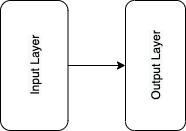
\includegraphics[width=0.4\linewidth]{Evaluation_Images/House_Prices_Architecture.png}
  \caption{Houses Prices model architecture}
  \label{fig:house-architecture}
\end{figure}
\subsection{LIME}
Figure \ref{fig:lime-house} is the explanation LIME provides for an area in Boston where the median price of housing was predicted to be \$19870. From this Figure we are able to deduce that the feature that had the largest negative impact on the median price of this area is the \% lower status of the population (LSTAT) which is the proportion of the population that is considered lower status in terms of either education or type of employment and can be measured as \emph{1/2 (proportion of adults without, some high school education and proportion of male workers classified as laborers)} \cite{HARRISON197881} and the feature which had the largest positive impact is the average number of rooms per dwelling (RM).
\begin  {figure}[!htpb]
  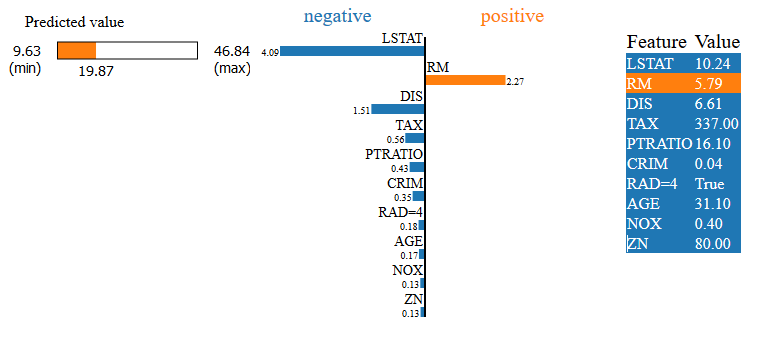
\includegraphics[width=\linewidth]{Evaluation_Images/House_LIME.png}
  \caption{LIME explanation for the predicted median price for an area in Boston.}
  \label{fig:lime-house}
\end{figure}
\subsection{SHAP}
Figure \ref{fig:shap-house-single} is the explanation SHAP provides for the same Boston area used in LIME. The base value in the figure is shown to be $22.89$ which is the average predicted value output over the entire training dataset. This can also be regarded as the models output given no input features. The figure highlights how each feature contributes to pushing the prediction from the base value. The red arrows are pushing towards the prediction which indicates that they increase the price and therefore have a positive impact. The blue arrows push against the prediction which indicates that they decrease the price and therefore have a negative impact. The explanation provided is a lot different to that of LIME's, because SHAP indicates how each feature either increases or decreases the prediction starting at the base value. An obvious difference between this and the SHAP explanation is that RM seems to have a negative impact on the price. This is due to the average RM being $6.28$ in the dataset and since this is below the average with $5.787$ it has an overall negative impact.
\begin  {figure}[!htpb]
  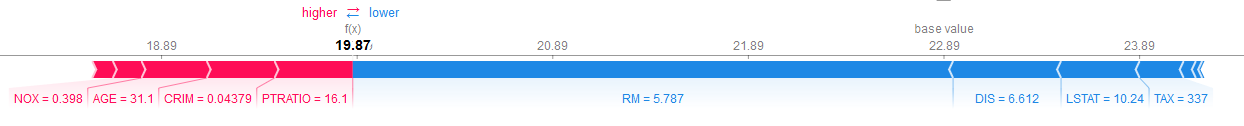
\includegraphics[width=\linewidth]{Evaluation_Images/house_indv_shap.png}
  \caption{SHAP explanation for the predicted median price for an area in Boston.}
  \label{fig:shap-house-single}
\end{figure}
Figure \ref{fig:shap-house-entire} is the explanation that SHAP provides over multiple different areas. This is known as a summary plot and it compares SHAP values of multiple instances and how their impact on the model prediction is related to the magnitude of that feature. Features which have larger SHAP values increased the median price where as those with smaller SHAP values decreased the median price.
\begin  {figure}[!htpb]
  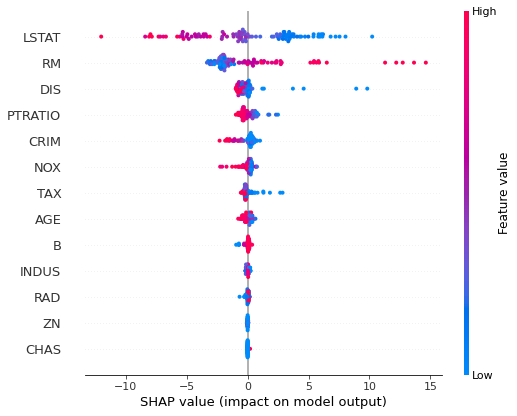
\includegraphics[width=\linewidth]{Evaluation_Images/house_shap.png}
  \caption{SHAP explanation over all the areas in Boston.}
  \label{fig:shap-house-entire}
\end{figure}
\subsection{Comparison}
Comparing LIME in Figure \ref{fig:lime-house} and SHAP in Figure \ref{fig:shap-house-single} which are the explanations of individual predictions they are largely similar. Both provide quantitative values for the effect each feature had on the prediction. SHAP, however explains how each feature affects the models average output given no input features. The largest advantage of SHAP is that the provided SHAP values are averaged over multiple instances known as background samples. SHAP is also able to easily visualize the SHAP values of multiple instances at a time as seen in Figure \ref{fig:shap-house-entire}.
\section{MNIST}

The MNIST digit classification problem is one of the most popular machine learning problems in image processing. The dataset consists of \emph{60000} training images and \emph{10000} test images of handwritten digits with a size of $28\times28$. The goal is to determine what digit class \emph{0-9} the specific image belongs to.
\subsection{Model Architecture} \label{sect:mnist-architecture}
For this problem we trained a Convolutional Neural Network (CNN). The architecture can be seen in Figure \ref{fig:mnist-architecture}. \emph{Convolutional Layers} are where features are extracted from our image, \emph{Max Pooling Layer} takes groups of values and changes them all to the maximum value among them, \emph{Dropout Layers} drop random weights between layers in order to prevent over-fitting, the \emph{Flatten layer} converts a matrix into a single flat array. The input is the image $28\times28$ and the output contains 10 values, each being a probability that the image belongs to a specific digit class.
\begin  {figure}[!htpb]
  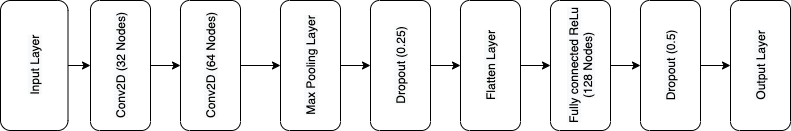
\includegraphics[width=\linewidth]{Evaluation_Images/mnist_architecture.png}
   \caption{Mnist model architecture.}
    \label{fig:mnist-architecture}
\end{figure}
\subsection{LIME}
Since there are $28 \times 28 = 784$ potential features, LIME creates a perturbed input $z^{'}$ by randomly choosing subsets of the non-zero features.  We limited the amount of perturbed samples generated by LIME to 1000 in order to increase the speed of the computation. In Figure \ref{fig:lime-mnist} we can see for the specific handwritten digit \emph{5}, the green pixels represents pixels which attributed towards predicting the that the digit is 5 and red pixels which attributed towards the digit being 3.
\begin  {figure}[!htpb]
  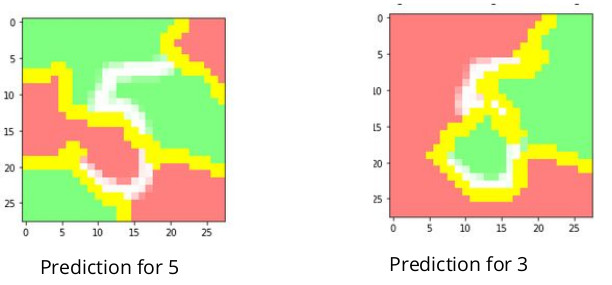
\includegraphics[width=\linewidth]{Evaluation_Images/Lime_mnist.jpg}
  \caption{Example of LIME visual feedback for the digit 5.}
  \label{fig:lime-mnist}
\end{figure}

\subsection{SHAP}
When making use of SHAP we are able to take an expectation of multiple samples which are referred to as \emph{background samples} in order to gain a more accurate representation of the attributed SHAP values. For this problem we took a set of 1000 background samples. In Figure \ref{fig:shap-mnist-3} we can see the SHAP explanation for the digit 3. Since our model provides a probability that the digit belongs to it for each class we are able to see which parts of the image added to that probability. The model gave the class 3 the highest probability with $34.701\%$. From the red pixels we can see that it mostly looked at the curves in the digit and the middle line to predict that it was the digit 3. From the blue pixels we can see that the inward curls at the end of the top and bottom curves decreased the probability. The second highest probability was the digit 2 with $21.261\%$ and once again we are able to see which pixels increased this probability and which decreased it. We have another example in Figure \ref{fig:shap-mnist-5} for the digit 5. Our model is much more certain in this example as we can see the probability of it belonging to class 5 is $64.285\%$. The red pixels also look a lot more intuitive as we can see that the model looked at the the top horizontal and vertical line, as well as the empty space below it to conclude that this is the digit 5.
\begin  {figure}[!htpb]
  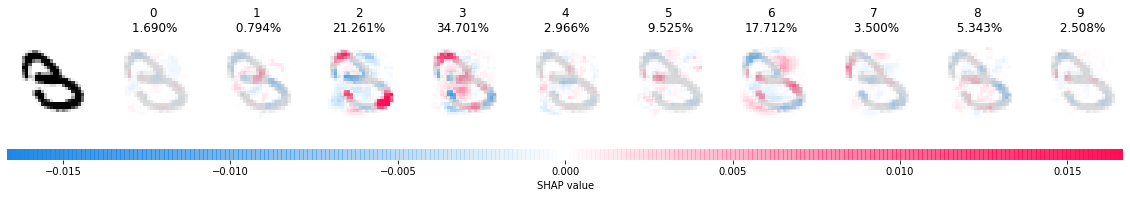
\includegraphics[width=\linewidth]{Evaluation_Images/shap_digit_3.png}
  \caption{SHAP values plotted for digit 3.}
  \label{fig:shap-mnist-3}
\end{figure}
\begin  {figure}[!htpb]
  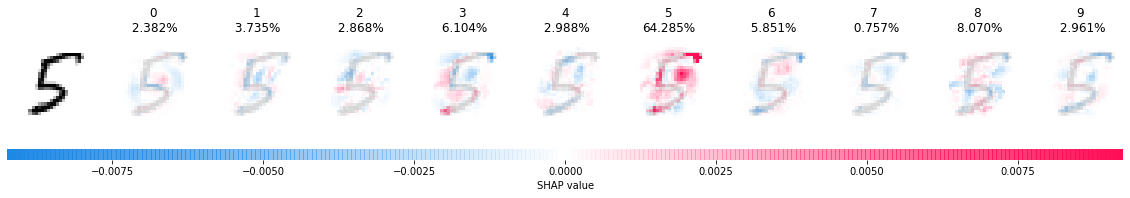
\includegraphics[width=\linewidth]{Evaluation_Images/shap_digit_5.png}
  \caption{SHAP values plotted for digit 3.}
  \label{fig:shap-mnist-5}
\end{figure}

\subsection{Lucid}
For Lucid we look at the spatial activations into two of the hidden convolutional layers labeled \emph{Conv1} and \emph{Conv2} respectively. Lucid provides a user interactive interface for viewing the activations, however in this example we will showcase static visual feedback. In Figure \ref{fig:lucid-mnist-3} we showcase the digit 3 and in Figure \ref{fig:lucid-mnist-5} the digit 5. For the two hidden layers \emph{Conv1} and \emph{Conv2} we are able to use spatial activations to see where and how much a specific set of pixels in the Conv1 Layer attributed in the target layer Conv2. The orange square is the set of pixels we are looking at in the starting layer and the whitened pixels in the target layer is where the activations happen

\begin  {figure}[!htpb]
  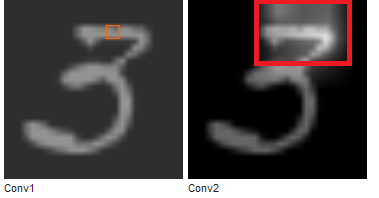
\includegraphics[width=\linewidth]{Evaluation_Images/LUCID_MNISTS_3.png}
  \caption{Lucid spatial activation for the digit 3.}
  \label{fig:lucid-mnist-3}
\end{figure} 
\begin  {figure}[!htpb]
  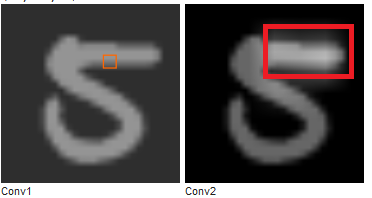
\includegraphics[width=\linewidth]{Evaluation_Images/LUCID_MNISTS_5.png}
  \caption{Lucid spatial activation for the digit 5.}
  \label{fig:lucid-mnist-5}
\end{figure} 
\subsection{Comparison} \label{sect:mnist-comparison}
Looking at the explanation that LIME produced in Figure \ref{fig:lime-mnist} it is quite clear which set of pixels had a positive and negative contribution for both the classes 5 and 3. Although it is easy to understand, it may be too simple, since by making use of super pixels we can't look at small sets or individual pixels but only large segments. SHAP on the other hand marks individual pixels which provides much more information into exactly which parts of the image attributed positively to which class. SHAP also provides the contribution that each pixel had with regards to the prediction which is the SHAP value magnitude as indicated by hue of the pixels. Lucid provides a completely different explanation. Rather then how the pixels contributed to each class, Lucid is able to explain between 2 layers which pixels from the source layer was responsible for activations in the destination layer. This provides intuition into how different layers interact with each other and can be valuable when attempting to understand the deeper inner workings of the network.
\section{Cats vs Dogs}

The Cats vs. Dogs is an image classification problem of finding suitable detectors for differentiating whether an image is of a cat or a dog. The dataset consists of 1000 \emph{training images} and  500 \emph{test images} with a size of $150\times150\times3$. 
\subsection{Model Architecture}
We also trained a CNN for this model and it's architecture can be seen in Figure \ref{fig:cats-dogs-architecture} which is similar to that of the MNIST problem in Section \ref{sect:mnist-architecture}. The input is the image matrix $150\times150\times3$ and the output is the probabilities of the image being a cat or dog.
\begin  {figure}[!htpb]
  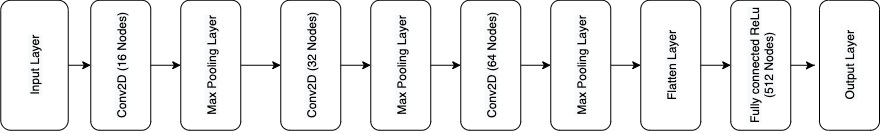
\includegraphics[width=\linewidth]{Evaluation_Images/Cats_Dogs_architecture.png}
   \caption{Cats and Dogs model architecture.}
    \label{fig:cats-dogs-architecture}
\end{figure}

\subsection{LIME}
 In Figure \ref{fig:lime-cat} we have an image of a cat and we visualize which super pixels attributed towards the \textbf{prediction of the image being a cat}, the green sections represent pixels that attributed positively towards it being a cat where as the red sections represent pixels which attributed positively towards it being a dog. As a human this seems to make some intuitive sense, the ears of the cat are marked as positive attributions due to the fact that we associate dogs with ``droopy ears'', where as the cat has ``fluffy ears''. Another example is in Figure \ref{fig:lime-cat-2} where our model \textbf{incorrectly identified the cat as a dog}, the image believes the ears don't belong to a dog since it can be seen as ``fluffy ears'' , however it believes that a large segment of the face belongs to a dog and overall it seems to be a stronger predictor than the ears and therefore the image was ultimately predicted to be a dog.
 
 \begin  {figure}[!htpb]
\centering
  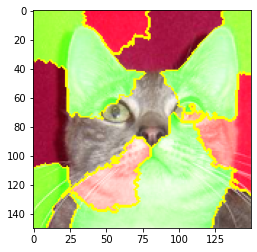
\includegraphics[width=0.8\linewidth]{Evaluation_Images/cats_explain_2.png}
  \caption{LIME explanation for the prediction of a cat.}
  \label{fig:lime-cat}
\end{figure}

\begin  {figure}[!htpb]
\centering
  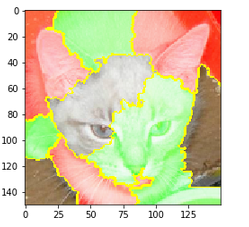
\includegraphics[width=0.8\linewidth]{Evaluation_Images/cats_explain.png}
  \caption{LIME explanation on an image of a cat which was falsely predicted to be a dog.}
  \label{fig:lime-cat-2}
\end{figure}

\subsection{SHAP}
In Figure \ref{fig:shap-cat} we show the SHAP values of 5 input samples and how they attributed towards whether the image is that of a cat or dog. SHAP provides much more detailed descriptions as each individual pixel is marked but LIME seems to be easier to understand as super-pixels are marked rather than individual ones. In figure \ref{fig:shap-cat} we can see the SHAP values for 5 samples. The middle column is the attribution values the prediction towards being a cat, where as the right column is the attribution for being a dog. Red indicates a positive attribution, where as blue indicates a negative prediction. Looking at this figure along with highlighting individual pixels SHAP also provides the prediction strength of the pixels which is their SHAP values.
\begin  {figure}[!htpb]
  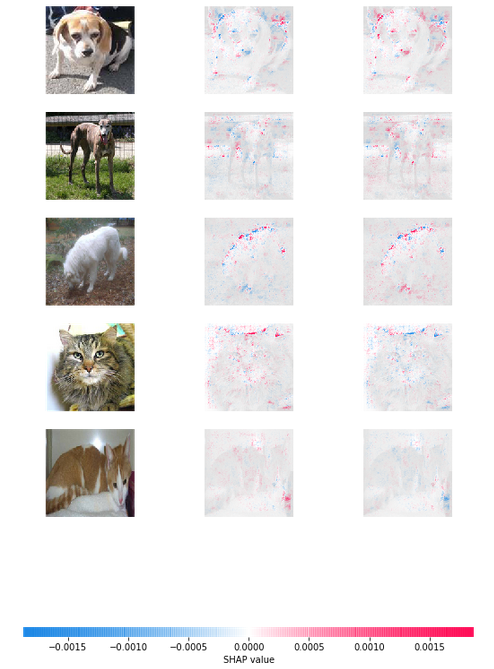
\includegraphics[width=\linewidth]{Evaluation_Images/CATS_DOGS_SHAP.png}
  \caption{Shap values for 5 different pictures of cats and dogs.}
  \label{fig:shap-cat}
\end{figure}

\subsection{Lucid}
In Figure \ref{fig:lucid-cat} we once again look at spatial activations between two hidden convolutional layers. However, in this case we included the gradient in the starting layer which shows the magnitude of the activations from the previous layers. In Figure \ref{fig:lucid-cat} for the two hidden layers \emph{Conv2} and \emph{Conv3} we are able to use spatial activations to see where and how much a specific set of pixels in the Conv2 Layer attributed in the target layer Conv3. The orange square is the set of pixels we are looking at in the starting layer and the whitened pixels in the target layer is where the activations happen.
\begin  {figure}[!htpb]
  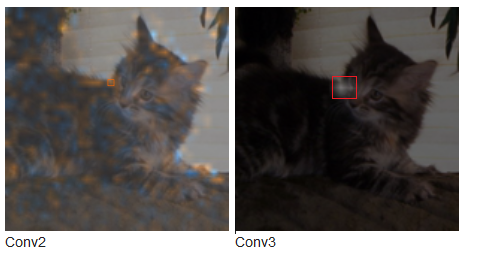
\includegraphics[width=\linewidth]{Evaluation_Images/LUCID_CATS_DOGS_2_v2.png}
  \caption{Lucid spatial activations between two layers in an image of a cat.}
  \label{fig:lucid-cat}
\end{figure}
\subsection{Comparison}
Since this is also a image-based model with similar architecture to the MNIST problem, the comparisons between the explanations provided by the tool are the same as those provided in Section \ref{sect:mnist-comparison}. LIME is easier to understand since it makes use of super-pixels, SHAP is more detailed as it marks individual pixels and also shows their magnitudes, where as Lucid provides analysis into the relationship between two layers.
\section{IMDB Sentiment analysis}
The goal of the \emph{IMDB sentiment analysis} problem is to classify whether a movie review is positive or negative. The dataset consists of 25000 \emph{training} samples and 25000 \emph{tests sample} where each sample is a vector of size $80\times1$. Each sample is a word embedding representing which words are present and in what order.
\subsection{Model Architecture}
For this problem we train a Recurrent Neural Network(RNN), the architecture can be seen in Figure \ref{fig:imdb-architecture}. The \emph{Embedding Layer} converts the input words into a vector representation that the model can understand, the \emph{Long Short-Term Memory (LSTM) layer} is a recurrent layer with feedback connections which is able to keep a history of previous words in the instance so that predictions take into account previous inputs. The output layer produces probabilities that the review is either negative or positive.
\begin  {figure}[!htpb]
\centering
  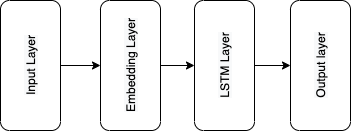
\includegraphics[width=0.5\linewidth]{Evaluation_Images/IMDB_Architecture.png}
   \caption{IMDB Sentiment analysis model architecture.}
    \label{fig:imdb-architecture}
\end{figure}
\subsection{LIME}
In Figure \ref{fig:lime-imdb} an attribution value is given to each individual word in the review, in this example we only show 8 words which had the largest impact. The model predicted that the review was positive with words such as ``great'', ``emotions'' and ``tears'' adding towards the review being positive and by human intuition these words can have positive connotations. Negative words such as ``wrong'' also have obvious negative connotations, however words such as ``half' or ``trying'' are not obviously negative and therefore some context is needed. Due to domain knowledge being needed, there is always some human interaction and if we have thousands of words that we are attributing on, it may become difficult to understand.
\begin  {figure}[!htpb]
  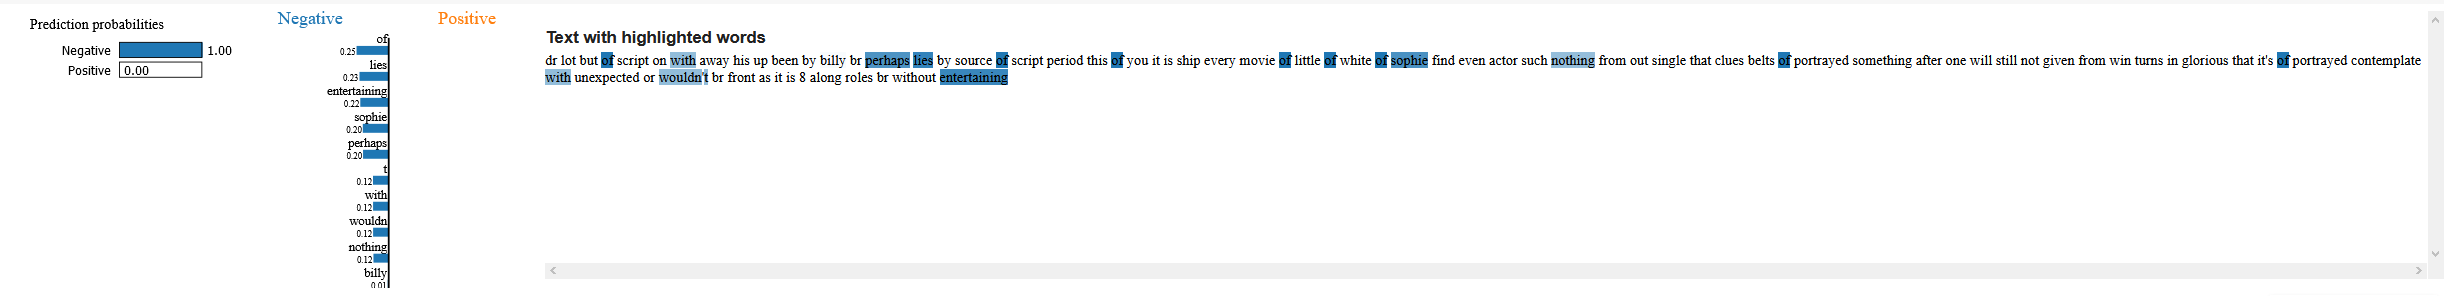
\includegraphics[width=0.75\linewidth]{Evaluation_Images/IMDB_explanation.png}
  \caption{The results of the attribution where the words which had the most impact towards the prediction are sorted by magnitude. Blue represents it being a negative attribution and orange represents positive.}
  \label{fig:lime-imdb}
\end{figure}


\subsection{SHAP}
In Figure \ref{fig:shap-imdb} we have chosen \emph{positive} to be the primary class of prediction. In this case SHAP orders the words by magnitude of attribution and the left side indicated words that attributed towards (increased the probability) of the primary class and the right side indicates words which attributed against (decreased the probability) the primary class. The output value for this particular case was 0.9 which means we have predicted that the review is positive. There are some obvious words which have positive connotation such as ``'laughs''. However none of the other words by human intuition are obviously good or bad if no other context is given. Therefore similar to LIME, knowledge of the domain and specific instance is needed to truly understand this explanation.

\begin  {figure}[!htpb]
  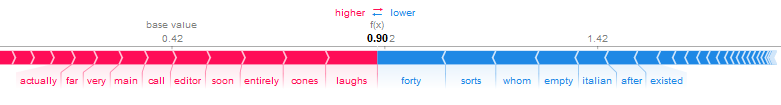
\includegraphics[width=\linewidth]{Evaluation_Images/IMDB_explanation_1.png}
  \caption{SHAP explanation for IMDB Sentiment analysis}
  \label{fig:shap-imdb}
\end{figure}
\subsection{Comparison}
Both the explanation of LIME in Figure \ref{fig:lime-imdb} and SHAP in Figure \ref{fig:shap-imdb} are similar in their explanations. The main difference being again that SHAP is averaging the SHAP values over multiple background samples. The SHAP explanation is also more compact and has a lot more clarity with regards to the effect of each feature on the prediction. However both tools face the same problem in that context and domain knowledge is needed to fully understand the problem.  Explanations which contain words without obvious positive or negative connotations and reviews which are sarcastic or satirical will not be easy to understand without the proper context. 
\section{Provide intuition into LIME and SHAP}

In this section we attempt to gain insight into how LIME and SHAP works by showing the relationship between a model with predefined weights and the produced feature attributions. 
\subsection{Setup}
 We start by creating a model with 5 weights which  are explicitly defined as,
\begin{align*}
w_1 = 5,\ w_2 = 3,\ w_3 = 4,\ w_4 = 9,\ w_5 = 1,
\end{align*}
in order to see the importance ratios between the weights we normalize them to unity,
\begin{align*}
    w_1 = 0.227, \ w_2 = 0.136, \ w_3 =  0.18 ,\ w_4 = 0.409, \ w_5 = 0.045.
\end{align*}
The next step is generating 500 synthetic data samples where each sample is an integer vector with 5 values between 1 and 100. We then assign each sample a probability of belonging to one of two respective classes \emph{Positive} and \emph{Negative} which are calculated as follows,
\begin{flalign*}
\begin{split}
\mbox{Sum(Positive)} &= X[0] \times w_1 + X[1] \times  w_2 + X[2] \times  w_3,
\\
\mbox{Sum(Negative)} &= X[3] \times  w_4 + X[4] \times  w_5 ,
\end{split}
\end{flalign*}
\begin{flalign*}
\begin{split}
\mbox{Prob(Positive)} &= \frac{Sum(Positive)}{Sum(Positive) + Sum(Negative)},
\\
\mbox{Prob(Negative)} &= \frac{Sum(Negative)}{Sum(Positive) + Sum(Negative)},
\end{split}
\end{flalign*}
where $X$ is the feature vector and $X[i]$ represents the feature at index $i$.
We pass this synthetic data to LIME and SHAP and observe how faithfully their produced feature attributions are to the actual weights.
\subsection{LIME}
Let $X_{1}$ and $X_{2}$ be 2 inputs with the following feature values,
\begin{flalign*}
\begin{split}
    X_1 &= [8,\ 24,\ 67,\ 87,\ 79],
    \\
    X_2 &= [48,\ 10,\ 94,\ 52,\ 98],
    \end{split}
\end{flalign*}
calculating the class probabilities for $X_1$,
\begin{flalign*}
\begin{split}
   \mbox{Prob(Positive)} &= 0.30595813,
    \\
    \mbox{Prob(Negative)} &= 0.6940418,
    \end{split}
\end{flalign*}
and for $X_2$,
\begin{flalign*}
\begin{split}
    \mbox{Prob(Positive)} &=  0.5330033 ,
    \\
    \mbox{Prob(Negative)} &= 0.4669967,
    \end{split}
\end{flalign*}
therefore $X_1$ belongs to the \emph{Negative} class and $X_2$ to the \emph{Positive} class.
We pass these two inputs to the Tabular Explainer of LIME in order to extract the feature attributions from the explanations. The visualization produced by LIME shows the feature attributions rounded to 2 significant digits, however for better accuracy the comparisons will use 3 significant digits. In Figure \ref{fig:lime-ground} we can see the attribution values which LIME assigns to each class for instance $X_1$,
\begin{align*}
    \phi_1 = 0.069, \ \phi_2 = 0.042, \ \phi_3 = 0.056 ,\ \phi_4 = 0.11, \ \phi_5 = 0.013,
\end{align*}
normalizing to unity,
\begin{align*}
    \phi_1 = 0.238, \ \phi_2 = 0.145, \ \phi_3 = 0.192 ,\ \phi_4 = 0.379, \ \phi_5 = 0.046.
\end{align*}
The explanation for $X_2$ can be seen in Figure \ref{fig:lime-ground2} and the attribution values are,
\begin{align*}
    \phi_1 = 0.061, \ \phi_2 = 0.036, \ \phi_3 = 0.048 ,\ \phi_4 = 0.126, \ \phi_5 = 0.014,
\end{align*}
normalizing to unity,
\begin{align*}
    \phi_1 = 0.215, \ \phi_2 = 0.127, \ \phi_3 = 0.167 ,\ \phi_4 = 0.441, \ \phi_5 = 0.05.
\end{align*}
\begin  {figure}[!htpb]
  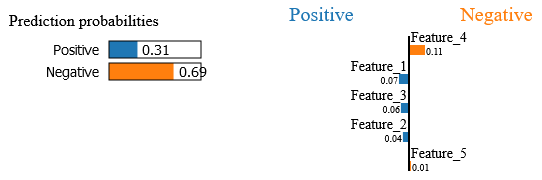
\includegraphics[width=\linewidth]{Evaluation_Images/lime-ground.png}
   \caption{LIME explanation for input $X_1$}
    \label{fig:lime-ground}
\end{figure}
\begin  {figure}[!htpb]
  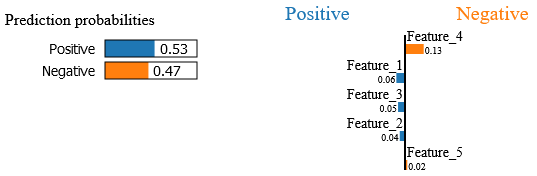
\includegraphics[width=\linewidth]{Evaluation_Images/lime-ground2.png}
   \caption{LIME explanation for input $X_2$}
    \label{fig:lime-ground2}
\end{figure}
A limitation of LIME that we have discussed before is that it only explains a single prediction at a time and we can see from the differences between the attributions values of $X_1$ and $X_2$  that there is variance between instances. This issue could be circumvented by  explaining multiple instances and averaging over the results.


\subsection{SHAP}
SHAP allows us to use the entire training set of 500 samples as background samples and gain attribution values which are averaged over the entire data set. We use \emph{Kernel SHAP} for this experiment since our model is not a Neural Network. The feature attribution values that we have derived from SHAP and normalized to unity are,
 \begin{align*}
    \phi_1 = 0.211, \ \phi_2 = 0.126, \ \phi_3 = 0.167 ,\ \phi_4 = 0.44, \ \phi_5 = 0.057.
\end{align*}
Figure \ref{fig:shap-ground} shows how each feature contributed towards the models prediction over the entire dataset for the \emph{Positive} class. The more red a point is the higher that particular feature value was, where as more blue indicates a lower value. The x-axis indicates the SHAP value, where the higher the value is the more that particular feature attributed towards the probability of the \emph{Positive} class and the lower it is the more it attributed against it. From this Figure we can see that Feature 1 to 3 attributed towards the \emph{Positive} class with Feature 1 attributing the most and Feature 2 the least. We can also see that Feature 4 attributed the most against it and Feature 5 the least. These results are inline with how we have defined the weights and from this graph we are able to visualize the different attributions between samples and their variances.
\begin  {figure}[!htpb]
  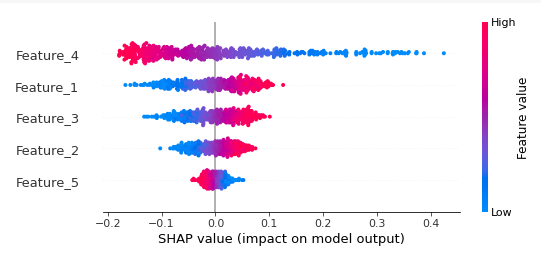
\includegraphics[width=\linewidth]{Evaluation_Images/shap_ground.png}
\caption{SHAP explanation for our chosen input $X_1$}
 \label{fig:shap-ground}
\end{figure}

\subsection{Comparison}
We have tabulated the results for comparison purposes in Figure \ref{fig:weight-tab}. We have also graphed the weights and attributions in Figure \ref{fig:weight-graph} for better visualization. We have also taken the average LIME attributions over the entire dataset in order to compare it to SHAP. We can see that the attribution values are fairly accurate in describing the defined weights and the ratios of feature importance are comparable to those of our model. From the results we have gathered, we can conclude that LIME and SHAP are able to generate fairly accurate linear estimations of a linear model by only using it's prediction results. These results allow us to gain some trust in LIME and SHAP, however further experimentation is needed to see if complex neural networks can also be approximated well.
\begin  {figure}[!htpb]
  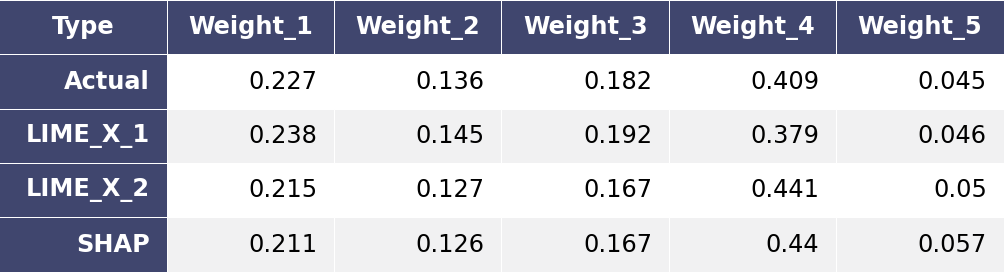
\includegraphics[width=\linewidth]{Evaluation_Images/weight_table.png}
   \caption{Comparison of weights.}
    \label{fig:weight-tab}
\end{figure}

\begin  {figure}[!htpb]
  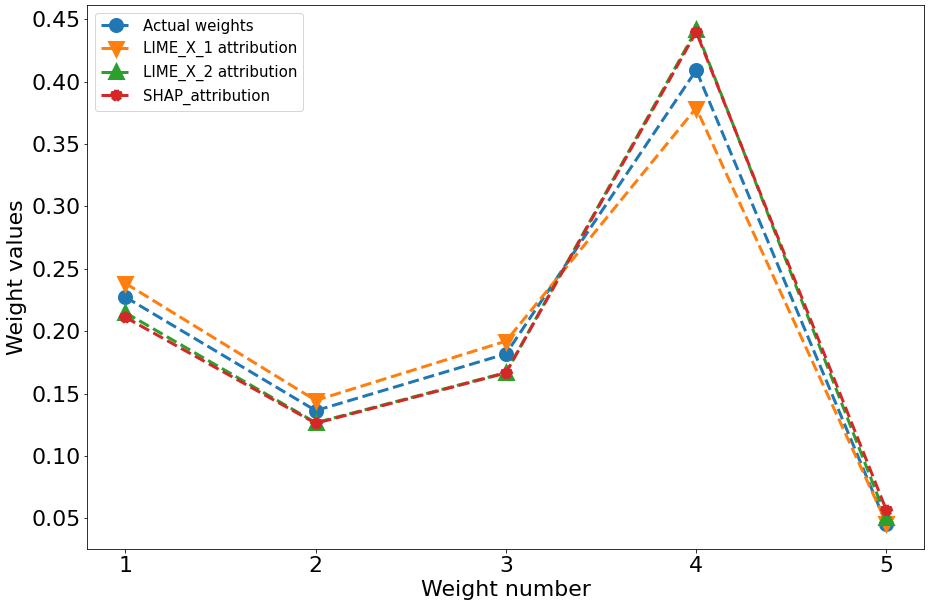
\includegraphics[width=\linewidth]{Evaluation_Images/weight_comp.png}
   \caption{Graph of weights.}
    \label{fig:weight-graph}
\end{figure}

\section{Conclusion}
From our evaluation we have shown that in all instances SHAP is superior to LIME in terms of the value that the explanations offer. In this thesis we are interested in how faithful these explanations are and therefore the extra computation of SHAP is not detrimental. One of the major advantages that SHAP has is that it is able to provide SHAP values that are averaged over multiple instances. This can somewhat be achieved with SP-LIME however it only chooses individual instances that are distinct from one another and the values are still calculated for each individual instance. Therefore we will solely be using SHAP to explain our Credit Loan Neural Network which we will discuss in the next Chapter.


